%! Author = Tom
%! Date = 07.12.2022
\chapter{Einleitung}

In diesem Kapitel führen wir an das Thema heran und stellen unsere Motive dar.
Wir definieren, welche Ziele wir in dieser Arbeit verfolgen und geben abschließend eine grobe Übersicht über die
Kapitelstruktur.

\section{Motivation}

Mit einer steigenden Nutzung von GraphQL wird es immer wichtiger, Tests für GraphQL-APIs zu entwickeln damit eine
gute Softwarequalität sichergestellt werden kann.
Die Entwicklung von Tests kann manuell oder automatisch geschehen.
Bei Unit-Tests, also Tests für einzelne Funktionen, kann ein Programmierer selbst entscheiden, ob er die Tests selbst schreiben will
oder sie von einem Tool automatisch generieren lasen will.
Integrations-Tests, also Tests die Kombinationen einzelner Interaktionen von Funktionen miteinander testen, hingegen haben sehr oft
einen sehr großen Testraum, sodass ein manuelles Schreiben dieser Tests fehleranfällig und langwierig ist.
Für REST-APIs existieren schon automatische Integrationstesttools wie zum Beispiel: EvoMaster \cite{evo-master} , QuickREST \cite{karlsson2019quickrest} oder RESTTESTGEN \cite{rest-test-gen}.
GraphQL-APIs haben leider noch einen Mangel an solchen automatischen Testtools.
Im Rahmen der internationalen  Konferenz für Automatisierung  von  Softwaretests IEEE/ACM 2021 wurde mit
\textit{Automatic Property-based Testing of GraphQL APIs}\cite{property-based-testing} eine Methode vorgestellt, die diesen Mangel angehen soll.
Es wurde eine Methode entwickelt die aus dem GraphQL-Schema, also der Beschreibung der Datenstruktur der API, Tests zufällig generiert und damit versucht Fehler in der Programmierung zu finden.
Die entwickelte Methode arbeitet nach folgendem Prinzip:

\begin{figure}[h!]
    \centering
    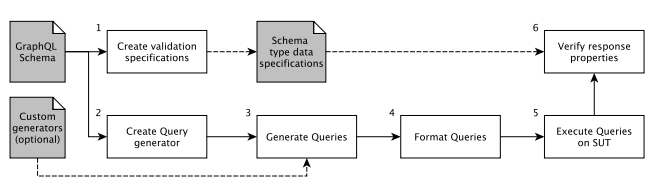
\includegraphics[width=\textwidth,height=\textheight,keepaspectratio]{content/einleitung/toolchain}
    \caption{Methode von~\cite{property-based-testing}}
    \label{property-based-method}
\end{figure}

Es wird aus einem GraphQL-Schema ein Query-Generator entwickelt.
Dieser kann aus der Typspezifikation, die GraphQL vorgibt, valide GraphQL-Querys entwickeln und diese anreichern mit verschiedenen Argumenten.
Die generierten Querys stellen die entwickelten Tests dar.
Das Besondere an GraphQL ist jedoch, dass es, wie der Name schon andeutet, einen Graphen umsetzt.
Ein sehr einfaches Schema lässt sich beispielhaft in diesen Graphen übersetzen:

\begin{figure}[h!]
    \centering
    % Linke Seite: Code
    \begin{minipage}{0.45\textwidth}
        \begin{lstlisting}[language=GraphQL]
  type Query {
    book(id: ID): Book
  }

  type Book {
    id: ID
    title: String
    sequel: Book
  }
        \end{lstlisting}
    \end{minipage}
    \hfill % Fügt horizontalen Abstand zwischen den Minipages hinzu
    % Rechte Seite: Grafik
    \begin{minipage}{0.45\textwidth}
        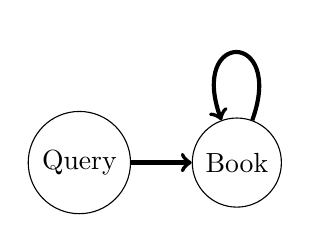
\begin{tikzpicture}
            \node[circle, draw] (n1) at (0,0) {Query};
            \node[circle, draw] (n2) at (2,0) {Book};

            \draw[->, line width=1.5pt] (n1) -- (n2);
            \draw[->, line width=1.5pt, looseness=8] (n2) to[out=70, in=110] (n2);
        \end{tikzpicture}
    \end{minipage}
    \caption{Schema zu Graph}
\end{figure}

Generell starten alle GraphQL-Querys im Query-Type.
Erlaubte Anfragen sind dann alle Pfade mit Ursprung im Query Knoten wobei Limitierungen implementiert werden können.
Property-based Testing nimmt nun die definierten Felder im Query-Type und geht die Pfade welche sich im Graphen ergeben zufällig ab.
Nach einer bestimmten Anzahl an zufälligen Iterationen wird die Query aus dem erlangten Pfad generiert und ausgeführt.
Nutzen wir nun jedoch ein wesentlich größeres Schema, zum Beispiel die GraphQL-API von GitLab~\cite{gitlab} so erkennt man schnell, dass
der Graph so komplex wird, dass eine zufällige Pfadgenerierung zu unzuverlässig und ineffizient ist um
eine große Struktur zuverlässlich zu testen.


TODO:
- Auf Graphstruktur zu sprechen kommen
- Hinleitung auf Graphen als Kontrollflussgraphen
- Graphcoverage Kriterien
- Anwendung an GraphQL zeigen
- Motivation abschließen









Die vorgestellte Methode bezieht sich auf ''Property-based Testing'' wobei diese gleichzusetzen ist mit ''Random Testing'' \cite{property-based-testing}[vgl. 2.B]
Durch die starke Typisierung und Schema-Definition, welche prinzipiell ein Graph ist, lässt sich in GraphQL
sehr einfach auswerten welche Anfragen nun zulässig sind.
Die hier vorgestellte Methode nutzt den Fakt, dass zum Beispiel alle möglichen Anfragen immer im Query-Knoten
beginnen müssen und somit alle weitergehenden Felder im Schema innerhalb des Query-Knoten definiert sein müssen.
Da die Definition des Schemas der eines Graphens entspricht ist jedoch der mögliche Suchraum potentiell unendlich da GraphQL
Zyklen innerhalb des Graphens erlaubt.
Der unendliche Suchraum wurde durch ein Rekursionslimit begrenzt allerdings wird so eine schlechtere Test-Coverage erreicht.
\newpage
Die bisher entwickelte Methode funktioniert auf folgende Weise:



wobei neben dem vorher erwähnten Rekursionslimit außerdem Punkt 6. ''Verify response Properties'' kritisch
zu betrachten ist da die Auswertung wirklich nur auf die Properties schaut.
Dies bedeutet, dass ein zurückgegebens Objekt nur auf seinen Typ überprüft wird aber nicht, ob seine tatsächlichen Rückgabewerte, die exakt erwartet sind.
Hierdurch können false-positives entstehen.

Die vorgestellte Methode wollen wir verbessern durch Änderung einiger Ansätze.
Hierbei sollen Graphcoverage-Algorithmen zum Einsatz kommen, die mit iterativen Verfahren auch zyklische Graphen ideal
überdecken können und dabei immer verlässlich arbeiten, sodass die generierten Tests stets für vergleichbare Ergebnisse sorgen und nicht
davon abhängig sind, dass der Zufall eine gute Überdeckung liefert.
Zusammenfassend sei gesagt, dass bei der Testgenerierung und Testauswertung Verbesserungen möglich sind und dies Gegenstand dieser Arbeit sein soll.













































\section{Umsetzung}

Zuallererst wird in dieser Arbeit etwas Theorie definiert und in Bezug gesetzt.
Wir beginnen damit die Graphentheorie als mathematisches Konzept zu definieren denn dieses liegt GraphQL zugrunde.
Darauffolgend kommt eine kleine Einführung in GraphQL und dann bilden wir schon die Schnittstelle von GraphQL zur Graphentheorie.
Sobald diese Verbindung erfolgt ist können wir uns dem eigentlichen Problem widmen: Wie kann man mithilfe von Graphcoverage-Algorithmen
Tests generieren?
Hierfür erfolgt ein letzter Theorie-Exkurs über Software-Tests.
Mit diesen Grundlagen schaffen wir es dann unsere Methode zu entwickeln und können Sie auch mit ''Automatic Property-based Testing of GraphQL APIs''\cite{property-based-testing}
vergleichen.
Unsere Methode wird konzeptionell vorgestellt und dann folgen einige Implementierungsdetails sowie ein Vergleich beider Tools durch Experimente.
Abschließen wird die Arbeit mit einem Ausblick für zukünftige Arbeit und einem Fazit über unsere erreichten Verbesserungen.